\documentclass[russian, utf8]{eskdtext}
\newcommand*{\No}{\textnumero}
\ESKDdepartment{Кафедра Систем Управления и Информатики}
\ESKDcompany{Университет ИТМО}
\ESKDdocName{ПОЯСНИТЕЛЬНАЯ ЗАПИСКА}
\ESKDsignature{КСУИ.207.435.001 ПЗ}
\ESKDauthor{Овчаров А.О.}

\usepackage{tocloft}
\renewcommand{\cftaftertoctitle}{\hfill}
\renewcommand{\cfttoctitlefont}{\hspace{7cm}\Large\bfseries}    %KOSTIL'
\renewcommand{\cftaftertoctitle}{\hfill}
\renewcommand{\cftdot}{.}
\renewcommand{\cftsecleader}{\cftdotfill{\cftdotsep}} % for sections
\makeatletter

\usepackage{pgfplots}
\usepgfplotslibrary{polar}
\pgfplotsset{compat=1.13}
\pgfplotsset{grid = major, grid style = {dashed}}

\usepackage{subcaption}
\usepackage{amsmath}
\usepackage{amsbsy}

\usepackage{float}

% PGFPlots Table ========================================================
\usepackage{pgfplotstable}
\renewcommand{\arraystretch}{1.3}
% recommended:
\usepackage{booktabs}
\usepackage{colortbl}
% pgfplotstable settings
\pgfplotstableset{
    every head row/.style = {before row = \hline},
    after row = {[1mm] \hline},
    column type = {|c},
    every last column/.style={
        column type/.add={}{|},
    },   
}
\usepackage{threeparttable}
\renewcommand{\TPTminimum}{0.6\linewidth}

% Paragraph indent
\usepackage{indentfirst}
\setlength{\parindent}{15mm}

%Change label separator
\usepackage{caption}
\captionsetup[table]{labelformat=simple, labelsep = endash, justification = raggedright, singlelinecheck = off, width = 0.75\textwidth}
\captionsetup[figure]{labelformat=simple, labelsep = endash, name = Рисунок}

\newcommand*{\tline}[2]{$\underset{\text{#1}}{\text{\underline{\hspace{#2}}}}$}

\begin{document}
\tableofcontents
\thispagestyle{empty}
\newpage

\section*{Введение}
\addcontentsline{toc}{section}{Введение}

В данной работе мы синтезируем регулятор методом коррекции ЛАЧХ. Выполяется построение желаемой ЛАЧХ разомкнутой системы на основе ЛАЧХ неизменяемой части и заданных показателей качества. \par
Построение желаемой характерисики разбивается на три части: низкочастотную, среднечастотную и высокочастонтую. Высокочастотная часть не оказывает никакого влияния на систему. Среднечастотная и низкочастотная части влияют на время пререхоного процесса, запас устойчивости по фазе и амплитуде и соотвественно на перерегулирование. \par
После построения желаемой ЛАЧХ системы, мы можем найти передаточную функцию регулятора, выполняющего "коррекцию" неизменяемой части системы в соотвествии с заданными показаетелями качества.

\newpage

\section{Постановка задачи}

Задан объект управления, описание которого определяется Wнч(s) – передаточной функцией неизменяемой части системы. Структурная схема следящей системы представлена на рисунке 1.

\begin{figure}[h!]
\centering
\begin{tikzpicture}
    %\draw[step=1cm,gray,very thin] (0, 0) grid (8,4);
    \draw[thick, ->](0, 3) -- (0.75, 3) node[anchor = south east] {g};
    \draw[thick] (1, 3) circle (0.25); \draw[fill] (1, 3) -- (1.18, 2.82) arc (315:225:0.25) -- (1, 3);
    \draw[thick] (0.82, 2.82) -- (1.18, 3.18); \draw (0.82, 3.18) -- (1.18, 2.82);
    \draw[thick, ->] (1.25, 3) -- (2, 3);
    \draw[thick] (2, 2.5) -- (2, 3.5) -- (4, 3.5) -- (4, 2.5) -- (2, 2.5);
    \draw (3, 3) node {$W_\text{рег}(s)$};
    \draw[thick, ->] (4, 3) -- (5, 3);
    \draw[thick] (5, 2.5) -- (5, 3.5) -- (7, 3.5) -- (7, 2.5) -- (5, 2.5);
    \draw (6, 3) node {$W_\text{нч}(s)$};
    \draw[thick, ->] (7, 3) -- (8, 3) node[anchor = south east] {y};
    \draw[fill] (7.5, 3) circle (0.07);
    \draw[thick, ->] (7.5, 3) -- (7.5, 1.5) -- (1, 1.5) -- (1, 2.75);
\end{tikzpicture}
\caption{Структурная схема проектируемой следящей системы}
\end{figure}

Требуется спроектировать регулятор, включенный последовательно с неизменяемой частью (нч) системы в контуре ошибки, с передаточной функцией $W_\text{рег}(s)$, который обеспечивает в замкнутой следящей системе с единичной обратной связью заданый набор показателей качества. Показатели качества указаны в таблице 1. \par
\begin{table}[h!]
    \centering
    \begin{threeparttable}        
        \caption{Данные}
        \def\arraystretch{2}
        \begin{tabular} {|c|c|c|c|c|c|c|c|c|}
            \hline
            $W_\text{нч}(s)$ & K & $T_1$ & $T_2$ & $t_\text{п}$ & $\sigma$ & $g_{max}$ & $g_{0max}$ & $e_{max}$ \\ \hline 
            $\displaystyle\frac{K}{(T_1s + 1)(T_2s + 1)s}$ & 210 & 0.04 & 0.2 & 0.1 & 27 & 5 & 0.8 & 0.015 \\ [2mm] \hline 
        \end{tabular}
    \end{threeparttable}
\end{table}
Здесь
K - коэффициент передачи неизменяемой части системы;
$T_1$, $T_2$ - постоянные времени (сек.);
$t_\text{п}$ - время переходного процесса (сек.);
$\sigma$ - перерегулирование (\%);
$g_{max}$ - максимально-допустимое значение скорости (м/с);
$g_{0max}$ - максимально-допустимое значение амплитуды гармонического сигнала;
$e_{max}$ - максимально-допустимое значение установившейся ошибки, \par

\newpage
\section{Анализ устойчивости неизменямой части}

Неизменяемая часть НЧ представлена передаточной функцией:
\begin{equation}
    W\text{нч} = \frac{210}{(0.04s + 1)(0.2s + 1)s} = \frac{210}{0.008s^3 + 0.24s^2 + s}
\end{equation}

Также найдем полюса передаточной функции (1) для оценки устойчивости системы, они представлены ниже:
\begin{align*}
    p_1 & = 0 & p_2 & = -25 & p_3 & = -5
\end{align*}

Соответственно по корневому критерию устойчивости система находится на границе устойчивости. Переходной процесс при нулевом входном воздействии и ненулевых начальных условиях ($y(0) = 1$) представлен на рисунке 2.

\begin{figure}[h!]
    \centering
    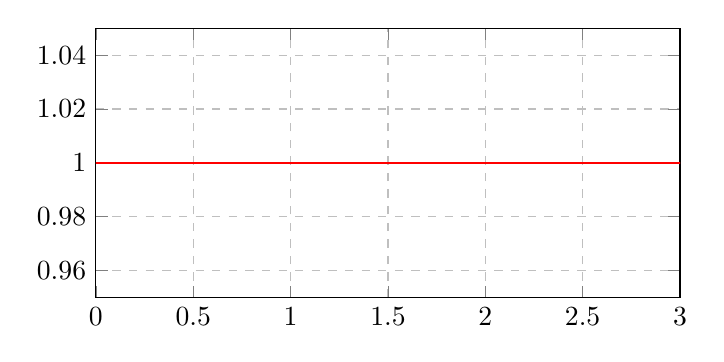
\begin{tikzpicture}
        \begin{axis} [
            height=9cm, width=9cm, grid=major,
            xmin = 0, height = 5cm, xmax = 3,
            ymin = 0.95, ymax = 1.05,
        ]
            \addplot[thick, red] {1};
        \end{axis}
    \end{tikzpicture}
    \caption{Переходная функция}
\end{figure}

Как видно из рисунка 2 и полюсов системы (1) системы находится на границе устойчивости нейтрального типа. Давайте замкнем единичной отрицательной обратной связью систему и проведен ее анализ. \par
Передаточная функция замкнутой системы выглядит следующим образом: 
\begin{equation*}
    W(s) = \frac{W\text{нч}}{W\text{нч} + 1} = \frac{210}{(0.04s + 1)(0.2s + 1)s + 210}
\end{equation*}
Раскрыв скобки получм: 
\begin{equation}
    W(s) = \frac{210}{0.008s^3 + 0.24s^2 + s + 210}
\end{equation}

\newpage
Для анализа устойчивости замкнутой системы построим матрицу гурвица на основании характеристического уравнения.
\begin{equation}
    H_3 = \begin{bmatrix}
        0.24 & 210 & 0 \\
        0.008 & 1 & 0 \\
        0 & 0.24 & 210
    \end{bmatrix}
\end{equation}

Нейдем главные миноры данной матрицы и воспользуемся критерием Гурвица.
\begin{align*}
    \Delta_1 & = 0.24 > 0 \\
    \Delta_2 & = -1.44 < 0 \\
    \Delta_3 & = -302.4 < 0
\end{align*}

В соответсвии с критерием гурвица, поскольку система имеет отрицательные миноры, она не устойчва. Это также можно увидеть, получив переходную характеристику замкнутой системы, которая изображена ниже. 

\begin{figure}[h!]
    \centering
    \begin{tikzpicture}
        \begin{axis} [
            xmin = 0, xmax = 1,
            width = 13cm, height = 7cm,
        ]
            \addplot[red, mark = none, thick] table {data/CloseSystemStep.csv};
        \end{axis}
    \end{tikzpicture}
    \caption{Переходной процесс замкнутой системы}
\end{figure}

\newpage
\section{Синтез регулятора}
Регулятор синтузируется методом коррекции ЛАЧХ, для чего нужно построить желаемую ЛАЧХ $L_\text{ж}$ и по ней найти желаемую передаточную функцию $W_\text{ж}$. Данная функция ПФ ялвяется произведением ПФ регулятори и незименяемой части (выражение 2). Из него можем выражить выражение для ПФ регулятора (выражение 3).\par
\begin{align}
    W_\text{ж} & = W_\text{рег}W_\text{нч} \\
    W_\text{рег} & = \frac{W_\text{ж}}{W_\text{нч}}
\end{align} \par
\subsection{Низкочастотный участок ЛАЧХ}
Для системы с астатизмом первого порядка первая низкочастотная асимптота проводится так, чтобы она имела наклон -20 дБ/дек и пересекала желаемую добротность по скорости $K_d$. При этом вся низкочастотная часть не должна пересекать запрещенную зону, которая формируется из желаемой добротности по скорости $K_v$ и критичксокй частоты гармонического сигнала $\omega_k$.\par
Давайте найдем все необходимые параметы запретной зоны:
\begin{align} 
    K_v &= \frac{g_{max}}{e_{max}} \approx 333.33 \\
    \omega_k & = \frac{g_{max}}{g_{0max}} = 6.25
\end{align} \par

Для упрощения регулятора можно выбрать сопрягающую частоту $\omega_1 = 1/T_2 = 5$, тогда необходимо увеличить желаемую добротность по скорости. Давайте найдем $K_d$, учитывая $\omega_1$.
\begin{equation}
    K_d = K_v\omega_kT_2 \approx 416.67
\end{equation}

\subsection{Среднечастотный участок ЛАЧХ}
Среднечастотный участок желаемой ЛАЧХ образуется асимптотой с наклоном -20 дБ/дек, проводимой так, чтобы она пересекала ось частот при $\omega_c$. Этот участок проводится влево и вправо до достижения модулей, равных $L_1$ и $L_2$. Затем производится сопряжение средпечастотного участка с низкочастотными асимптотами и высокочастотной частью. Для нахождения частоты среза $\omega_c$ необходимо найти частоту положительности $\omega_\text{п}$, которую можно найти соотвественно из диаграмм в учебнике Бесекерского (выражение 5, 6).
\begin{align}
    \omega_\text{п}|_{\sigma = 27\%} & = \frac{4\pi}{t_\text{п}} \approx 125.66\ \frac{1}{c} \\
    \omega_c & = 0.9\omega_\text{п} \approx 113.1\ \frac{1}{c} 
\end{align}
Амплитуды $L_1$ и $L_2$ также находятся по диаграммам в учебнике Бесекерского исходя из заданных показателей качества. В нашем случае они имеют следующие значения:
\begin{align*}
    L_1 & = 18\ \text{дБ} & L_2 & = -18\ \text{дБ}
\end{align*}
Для качественнго выполнения заданных показателей качества среднечастотаня асимтота может превышать данные значения по модулю, но не наоборот. \par
Для сопряжения среднечастотного участка и низкочастотного строится прямая, имеющая накол 40 - 60 дБ/дек. Эта прямая определяется сопрягающими частотами $\omega_1$, $\omega_2$. Из пересечения среднечастотной асимптоты и сопрягающей можем найти $\omega_2$.
\begin{equation}
    \omega_2 = \sqrt{\frac{K_dw_1^2}{w_c}} \approx 9.6
\end{equation}\par

\subsection{Высокочастотный участок}
Данный участок не вносит большого вклада в показатели качества, поэтому его выбирают максимально удобным для составления регулятора.
Теперь только осталось найти сопрягающую частоту $\omega_{3}$:
\begin{equation}
    \omega_{3} = \frac{\omega_c}{10^{L_2/20}} \approx 898.36\ \frac{1}{c}
\end{equation}

По найденым ниже параметрам можем построить желаемую ЛАЧХ, изображенную на рисунке ниже.

\begin{figure}[h!]
    \centering
    \begin{tikzpicture}
        \begin{semilogxaxis} [
            height=9cm, width=16cm, grid=major,
            ymin = -50, ymax = 75,
            xmin = 10e-1, xmax = 10e+3,
            xlabel = {$\omega$, 1/c},
            ylabel = {$L(\omega)$, дБ},
            %ytick = {-40, 0, 60},
            %extra y ticks = {46.44, 50.46, 32.47, 36.48, 22.4, 4.51, -19},
            %every extra y tick/.style = {
            %    yticklabel style={
            %        font = \tiny,
            %    },
            %}
        ]
            %\draw[fill = gray, dashed] (1, 50.46) -- (6.25, 34.54) -- (6.25, -50) -- (1, -50) -- (1, 50.46);
            \addplot[thick, blue, mark = *, mark options = {black}] coordinates {(1, 52.4) (5, 38.42) (9.5971, 21.4263) (898.36, -18) (3.0675e+03, -50)};

            \draw[fill] (1, 52.4) node[anchor = south west] {\scriptsize \textbf{(1, 52.4)}};
            \draw[fill] (5, 38.42) node[anchor = south west] {\scriptsize \textbf{(5, 38.42)}};
            \draw[fill] (9.6, 21.43) node[anchor = south west] {\scriptsize \textbf{(9.6, 21.43)}}; 
            \draw[fill] (898.36, -18) node[anchor = south west] {\scriptsize \textbf{(898.36, -18)}}; 
            \draw[fill] (113.0973, 0) circle (0.07cm) node[anchor = south west] {\scriptsize \textbf{(113.0973, 0)}};

            %\draw[dotted, thick] (1, 46.4444) -- (0.1, 46.4444);
            %\draw[dotted, thick] (1, 50.4576) -- (0.1, 50.4576);
            %\draw[dotted, thick] (5, 32.4650) -- (0.1, 32.4650); \draw[dotted, thick] (5, 36.4782) -- (5, -50);
            %\draw[dotted, thick] (5, 36.4782) -- (0.1, 36.4782);
            %\draw[dotted, thick] (8.58, 22.395) -- (0.1, 22.395); \draw[dotted, thick] (8.58, 22.395) -- (8.58, -50);
            %\draw[dotted, thick] (25, 4.5062) -- (0.1, 4.5062); \draw[dotted, thick] (25, 4.5062) -- (25, -50);

            

            \draw[dashed, thick] (0.1, 0) -- (10e+4, 0);
            %\draw[dotted, thick] (1.0080e+03, -19) -- (0.1, -19);

            %\legend{$L_\text{нч}$, $L_\text{ж}$};
        \end{semilogxaxis}
    \end{tikzpicture}
    \caption{ЛАЧХ}
\end{figure}

Теперь можем построить передаточную функцию желаемой системы:
\begin{equation}
    W_\text{ж} = \frac{K_d\left(\frac{1}{\omega_2}s + 1\right)^2}{s(T_2s + 1)^2\left(\frac{1}{\omega_3}s + 1\right)^2}
\end{equation} \par
И соответсвенно передаточную функцию регулятора:
\begin{equation}
    W_\text{рег} = \frac{K_d/K\left(\frac{1}{\omega_2}s + 1\right)^2(T_1s + 1)}{\left(\frac{1}{\omega_3}s + 1\right)^2(T_2s + 1)}
\end{equation} \par

\newpage
\section{Проверочный расчет}
Выполним проверочный расчет на заданные показатели качества. А именно посчитаем предельное значение ошибки при линейно возрастающем воздействии со скоростью $g_{max}$.
\begin{align*}
    \varepsilon_1 & = \left.\frac{1}{1 + W_\text{ж}(s)}G(s)\right|_{s\rightarrow0} = \\
    & = \left.\frac{s(T_2s + 1)^2\left(\frac{1}{\omega_3}s + 1\right)^2}{s(T_2s + 1)^2\left(\frac{1}{\omega_3}s + 1\right)^2 + K_d\left(\frac{1}{\omega_2}s + 1\right)^2}\frac{g_{max}}{s}\right|_{s\rightarrow 0} = \frac{g_{max}}{K_d} = 0.012 < e_{max}
\end{align*} \par
Теперь нужно убедиться, что разомкнутая система обладает достаточным запасом устойчивости по фазе и амплитуде.
\begin{align}
    \mu & =  180 - 90 - 2\arctg{\frac{\omega_c}{\omega_3}} - 2\arctg{\omega_c T_2} + 2\arctg{\frac{\omega_c}{\omega_2}} \approx 90^\circ \\
    L & = 23.8\text{ дБ}
\end{align}
где $\mu$ - запас по фазе, $L$ - запас по амплитуде при частоте $\omega = 889$ 1/c. \par
Осталось проверить качество выполнения перерегулирования и 

\newpage
\section{Реализация регулятора}

На рисунке ниже представлена электрическая схема передаточной функции регулятора.
\begin{figure}[h!]
    \centering
    \includegraphics {images/PrincipScheme.pdf}
    \caption{Принципиальная схема регулятора}
\end{figure}

Давайте покажем, что указанная схема действительно представляет регулятор. Условно схему можно резделить на 3 части. Первые две идентичны. Давайте составим передаточную функцию первой части ($U_1$ - $R_1 || C_1$ - $R_2$ - $U_1$), тогда не сложно будет представить и функцию всей системы. Выпишем первое и второе правила Кирхгофа:

\begin{equation*}
    \begin{cases}
        I_{R_2} = I_{R_1} + C_1\frac{dU_{C_1}}{dt} \\
        I_{R_1}R_1 = U_{C_1} \\
        U_1 = U_{C_1} + U_{R_2}
    \end{cases}
    \Leftrightarrow
    \begin{cases}
        I_{R_2} = \frac{U_{C_1}}{R_1} + C_1\frac{dU_{C_1}}{dt} \\
        I_{R_1} = \frac{U_{C_1}}{R_1} \\
        U_1 = U_{C_1} + I_{R_2}R_2 \\
        U_{R_2} = I_{R_2}R_2
    \end{cases}
\end{equation*}
из полученной системы можем выразить отдельно $U_1$ и $U_{R_2}$:
\begin{equation*}
    \begin{cases}
        U_1 = U_{C_1} + \frac{R_2}{R_1}U_{C_1} + R_2C_1\frac{dU_{C_1}}{dt} \\
        U_{R_2} = \frac{R_2}{R_1}U_{C_1} + R_2C_1\frac{dU_{C_1}}{dt}
    \end{cases}
\end{equation*} \par
Полученное выражение теперь представим в операторном виде:
\begin{equation*}
    \begin{cases}
        U_1 = \left( 1 + \frac{R_2}{R_1} + R_2C_1p \right) U_{C_1} \\
        U_{R_2} = \left( \frac{R_2}{R_1} + R_2C_1p \right) U_{C_1}
    \end{cases}
\end{equation*} \par

Остается только найти саму передаточную функцию: \par
\begin{equation}
    W_1(p) = \frac{U_{R_2}}{U_1} = \frac{\frac{R_2}{R_1} + R_2C_1p}{1 + \frac{R_2}{R_1} + R_2C_1p} = \frac{\frac{R_2}{R_1 + R_2}\left( R_1C_1p + 1 \right)}{\left( \frac{R_1R_2}{R_1 + R_2}C_1p + 1 \right)}
\end{equation}

Передаточная функция $W_2(p)$ аналогична первой. Теперь рассмотрим часть, содержащую операционный усилитель. Запишем выражения для входного $U_{R_2}$ и выходного $U_2$ напряжения.
\begin{align*}
    U_{R_2} & = \frac{R_3}{R_3C_2 p + 1} \\
    U_2 & = -\frac{R_4}{R_4C_3 p + 1}
\end{align*}
В итоге получи передаточную функцию:
\begin{equation}
    W_3(p) = -\frac{R_4/R_3(R_3 C_2 p + 1)}{R_4C_3 p + 1}
\end{equation}
Как видно, из выражения (18), последняя часть регулятора инвертирует входной сигнал. Далее вход объекта управления будет подключаться инверсно к выходу регулятора.

Теперь можем записать итоговое выражения для передаточной функции регулятора:
\begin{equation}
    W(p) = \frac{U_2}{U_1} = \frac{K\left(T_1p + 1 \right)^2 \left( T_3p + 1 \right)}{\left( T_2p + 1 \right)^2 \left( T_4p + 1 \ \right)} 
\end{equation}
\begin{align}
    K & = \frac{R_2^2R_4}{(R_1 + R_2)^2R_3} \\
    T_1 & = R_1C_1 \\
    T_2 & = \frac{R_1R_2}{R_1 + R_2}C_1 \\
    T_3 & = R_3C_2 \\
    T_4 & = R_4C_3
\end{align}

\newpage
Поскольку в данном уравнении 7 неизвестных и 5 уравнений, зададим $C_1 = 10^{-6}$ Ф. Тогда можем найти $R_1$ и $R_2$.
\begin{align*}
    R_1 & = \frac{T_1}{C_1} \approx 104166 \text{ Ом}\\
    R_2 & = \frac{T_1T_2}{(T_1 - T_2)C_1} = 1125 \text{ Ом}\\
\end{align*}

Теперь выразим $R_3$ и $R_4$, подставив $C_3 = 10^{-9}$ Ф.
\begin{align*}
    R_3 & = \frac{T_3}{C_2} \\
    R_4 & = \frac{T_4}{C_3} = 2\cdot 10^8 \text{ Ом}
\end{align*}

Подставим все в выражение (19), получим:
\begin{align*}
    K & = 570967.85C_2 \Rightarrow C_2 = 3.48 \cdot 10^{-6} \text{ Ф}\\
    R_3 & \approx 11510 \text{ Ом}
\end{align*}

В итоге получим схему в Multisim, представленную ниже на рисунке.

\begin{figure}[h!]
    \centering
    \includegraphics{images/ElectricScheme.pdf}
    \caption{Принципиальная хема регулятора}
\end{figure}

\newpage

Тажке построим передаточную функцию данного регулятора в Matlab.
\begin{figure}[h!]
    \centering
    \includegraphics{images/regulator.pdf}
    \caption{Cхема регулятора в Matlab}
\end{figure}

Теперь для выполнения качественного сравенения представлим переходные характеристики системы, построенной в Matlab и системы в Multisim.

\begin{figure}[h!]
    \centering
    \begin{tikzpicture}

        \begin{axis}[%
            name=plot1,
            xmin = 0, xmax = 1.2,
            title style={at={(0.5,-0.3)},anchor=north,yshift=-0.1},
            title = {(a) Multisim},
            xlabel = {t, c}, ylabel = {y},
            width = 0.46\textwidth,
            extra y ticks = {1.78},
        ]
             \addplot[mark = none, red, smooth] table[x = t, y = y] {data/ElData2.dat};
        \end{axis}

        \begin{axis}[%
            name=plot2,
            at=(plot1.right of south east), anchor=left of south west,
            xmin = 0, xmax = 0.009,
            title style={at={(0.5,-0.3)},anchor=north,yshift=-0.1},
            title = {(b) Matlab},
            xlabel = {t, c}, ylabel = {y, B},
            width = 0.46\textwidth,
            extra y ticks = {1.98},
            ytick = {1000, 2000, 3000},
        ]
            \addplot[mark = none, red, smooth] table[x = t, y = y] {data/RegStep.dat};
        \end{axis}
    \end{tikzpicture}
    \caption{Переходная функция регулятора}
\end{figure}

Как видно из рисунка 8, переходной процесс в Matlab проходит много быстрее, чем при симуляции электрической схемы. Также сигнал на рисунке 8 (a) ограничен в пределах $\pm 12$ вольт из-за операционного усилителя. 

\newpage
\section{Математическое моделирование}

В ходе работы была построяна схема моделирования полученноой желаемой передаточной функции, она указана на рисунке ниже: 
\begin{figure}[h!]
    \centering
    \includegraphics {images/model.pdf} 
    \caption{Схема моделирования}
\end{figure} \par

В результате мы получили различные графики при линейно нарастающем входном воздействии и синусоидальном а также переходная функция.
\begin{figure}[h!]
    \centering
    \begin{tikzpicture}
        \begin{axis} [
            width = 0.7\textwidth,
            height = 0.5\textwidth,
            xmin = 0, ymin = 0,
            xmax = 0.3,
            scaled ticks=false,
            tick label style={/pgf/number format/fixed},
            extra y ticks = {1.0622},
        ]
            \addplot[red, mark = none, thick] table {data/step.csv};
            \draw[fill] (0.037, 1.0622) circle (0.07cm);
            \draw[fill] (0.061, 1.05) circle (0.07cm) node[anchor = south west] {\scriptsize \textbf{(0.06, 1.05)}};
        \end{axis}
    \end{tikzpicture}
    \caption{Переходная функция}
\end{figure} \par
Как видно из рисунка 6 были получены следующие показатели:
\begin{align*}
    t_\text{п} & = 0.06\text{ c} & \sigma & = 6\text{ \%}
\end{align*} \par

\newpage
Далее не рисунке 7 представлен график при линейно нарастающем входном воздействии, здесь $\pmb{\varepsilon} = 0.012$, как и получилось при проверочном расчете.

\begin{figure}[h!]
    \begin{subfigure} {0.5\textwidth}
        \begin{tikzpicture}
            \begin{axis} [
                xmin = 0, ymin = 0,
                xmax = 0.05,
                xlabel = {$t$, c},
                ylabel = {$y$},
                width = 0.9\textwidth,
                scaled ticks=false,
                tick label style={/pgf/number format/fixed}
            ]
                \addplot[red, mark = none, thick] table[x = t, y = y] {data/LinEncrease.csv};
            \end{axis}
        \end{tikzpicture}
    \end{subfigure}
    \begin{subfigure} {0.5\textwidth}
        \begin{tikzpicture}
            \begin{axis} [
                xmin = 0, ymin = 0,
                xmax = 0.3,
                xlabel = {$t$, c},
                ylabel = {$e$}, 
                extra y ticks = {0.012},
                extra y tick labels = {$\pmb{\varepsilon}$},
                width = 0.9\textwidth,
                scaled ticks=false,
                tick label style={/pgf/number format/fixed}
            ]
                \addplot[red, mark = none, thick] table[x = t, y = e] {data/LinEncrease.csv};
            \end{axis}
        \end{tikzpicture}
    \end{subfigure}
    \caption{Графики переходных процессов при $g = 5t$}
\end{figure}

Осталось рассмотреть реакцию системы на синусоидально воздействие $g = 0.8\sin{3t}$. Как видно из рисунка 8, при синусоидально воздействии и $\omega = 3$ ошибка меньше 0.015.
\begin{figure}[h!]
    \begin{subfigure} {0.5\textwidth}
        \begin{tikzpicture}
            \begin{axis} [
                xmin = 0,
                xmax = 5,
                xlabel = {$t$, c},
                ylabel = {$y$},
                width = 0.9\textwidth,
                scaled ticks=false,
                tick label style={/pgf/number format/fixed}
            ]
                \addplot[red, mark = none, thick] table[x = t, y = y] {data/Sin.csv};
            \end{axis}
        \end{tikzpicture}
    \end{subfigure}
    \begin{subfigure} {0.5\textwidth}
        \begin{tikzpicture}
            \begin{axis} [
                xmin = 0, ymin = -0.02,
                xmax = 5, ymax = 0.02,
                xlabel = {$t$, c},
                ylabel = {$e$}, 
                extra y ticks = {0.015, -0.015},
                extra y tick labels = {0.015, -0.015},
                width = 0.9\textwidth,
                scaled ticks=false,
                tick label style={/pgf/number format/fixed}
            ]
                \addplot[red, mark = none, thick] table[x = t, y = e] {data/Sin.csv};
            \end{axis}
        \end{tikzpicture}
    \end{subfigure}
    \caption{Графики переходных процессов при $g = 0.8\sin{3t}$}
\end{figure}

\newpage
\section*{Вывод}
В данной работе мы синетзировали регулятор, выполняющий заданные показатели качества. Для синтеза использовался метод коррекции ЛАЧХ, придуманные Солодовниковым В. В. В данном методе ЛАЧХ неизменяемой части корректируется таким образом, чтобы при реакции на ступенчатый сигнал, показатели качества не превышали заданных значений. \par
Как видно в проевочных расчетах и на рисунках 6, 7 и 8 данный регулятор успешно справляется со своими задачами. \par
При подаче на вход гармонического сигнала, его частота, помножанная на амплитуду не должны превышать значение $g_{max}$. \par
Также мы получили электрическую схему, характерезующую передаточную функцию.

\end{document}